\documentclass{beamer}
\usetheme{Madrid}
\usepackage{pifont}  % Подключаем пакет для использования \ding
\usepackage{tikz}
\usepackage{xcolor}
\usepackage[english]{babel}  % Подключение для автоматического переноса слов

\title{Osint Bot Presentation}
\author{CEO | Yana Anisimova}

\begin{document}

\frame{\titlepage}

\section{What's the problem? Our people may be working for the enemy without even realizing it}

\begin{frame}
    \frametitle{What's the problem? Our people may be working for the enemy without even realizing it}
    
    \begin{block}{Questions that arise when applying for a job}
        \begin{itemize}
            \item Is the company I am going to work for connected to the aggressor country?
            \item Is it a reliable company?
            \item Is it worth getting involved?
            \item Will I have problems because I work or worked for this company?
            \item Etc.
            \item How can I quickly check an employer?
        \end{itemize}
    \end{block}
    
\end{frame}

\section{Our answer is Osint Bot}

\begin{frame}
    \frametitle{Our answer is Osint Bot}
    
    \begin{block}{AI-based Telegram bot that checks employer using OSINT methods}
        \begin{itemize}
            \item Find job postings of your employer on .ru and .by websites
            \item Analyze employer connections with the aggressor country using OSINT methods
        \end{itemize}
    \end{block}
    
\end{frame}

\section{It takes just 3 simple steps to get started:}

\begin{frame}
    \frametitle{It takes just 3 simple steps to get started:}
    
    \begin{block}{Enter company, enter job title. Get results}
        % Здесь можно добавить больше информации, если необходимо
    \end{block}
    
\end{frame}


\section{Market size: Ukrainian and Friends of Ukraine}

\begin{frame}
    \frametitle{Market size: Ukrainian and Friends of Ukraine}

    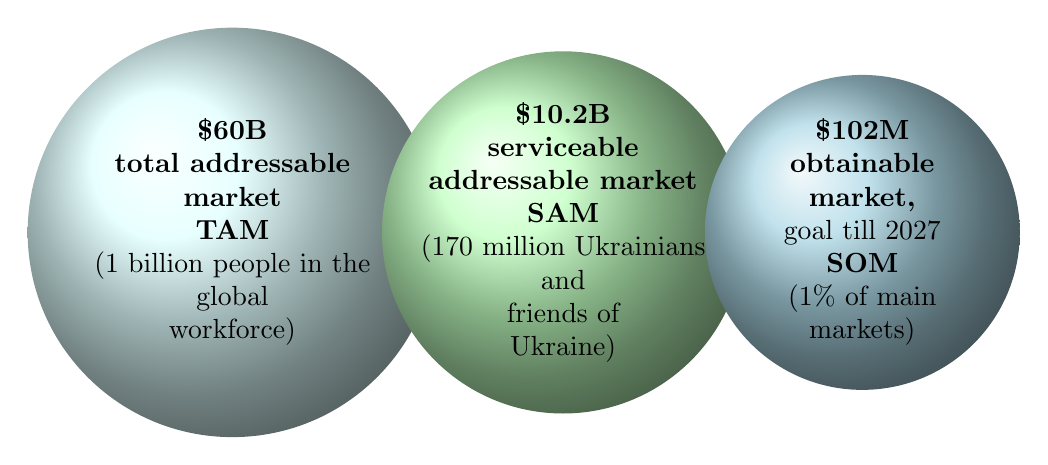
\begin{tikzpicture}

    % Colors for the circles
    \definecolor{lightblue}{RGB}{173,216,230}
    \definecolor{lightgreen}{RGB}{192,255,192}
    \definecolor{lightcyan}{RGB}{224,255,255}
    
    % TAM Circle
    \shade[ball color=lightcyan] (-11.7,0) circle (2.6cm);
    \node at (-11.7,0) {\parbox{4cm}{
        \centering
        \textbf{\$60B}\\
        \textbf{total addressable market}\\
        \textbf{TAM}\\
        (1 billion people in the global\\
        workforce)
    }};

    % SAM Circle
    \shade[ball color=lightgreen] (-7.5,0) circle (2.3cm);
    \node at (-7.5,0) {\parbox{4cm}{
        \centering
        \textbf{\$10.2B}\\
        \textbf{serviceable addressable market}\\
        \textbf{SAM}\\
        (170 million Ukrainians\\
        and\\
        friends of\\
        Ukraine)
    }};

    % SOM Circle
    \shade[ball color=lightblue] (-3.7,0) circle (2cm);
    \node at (-3.7,0) {\parbox{3cm}{
        \centering
        \textbf{\$102M}\\
        \textbf{obtainable market,}\\
        goal till 2027\\
        \textbf{SOM}\\
        (1\% of main markets)
    }};
    
    \end{tikzpicture}

\end{frame}


\section{How do we make money}

\begin{frame}
    \frametitle{How do we make money}
    
    \begin{block}{The bot will be in 2 versions:}
        \begin{itemize}
            \item Free version
            \item Subscription: \$5/month
        \end{itemize}
    \end{block}
    
\end{frame}


\section{Competition}

\begin{frame}
    \frametitle{Competition}
    
    \begin{block}{Competition}
        % Добавьте описание конкурентов
    \end{block}
    
\end{frame}

\section{Go to market strategy}

\begin{frame}
    \frametitle{Go to market strategy}
    
    \begin{block}{Go to market strategy}
        % Здесь можно описать стратегию выхода на рынок
    \end{block}
    
\end{frame}

\section{Our team}

\begin{frame}
    \frametitle{Our team}
    
    \begin{block}{}
        % Добавьте информацию о команде
        Yana Anisimova CEO 
        Yuriy Galych CTO
    \end{block}
    
\end{frame}

\section{Money raising}

\begin{frame}
    \frametitle{Money raising}
    
    \begin{block}{Money raising}
        % Добавьте описание стратегии привлечения средств
    \end{block}
    
\end{frame}


\section{OSINT bot invites investors to join us for peace in Ukraine and Europe}

\begin{frame}
    \frametitle{OSINT bot invites investors to join us for peace in Ukraine and Europe}
    
    \begin{block}{Join us for peace in Ukraine and Europe}
        % Добавьте описание предложения для инвесторов
    \end{block}
    
\end{frame}

\end{document}
